% В этом файле вы описываете задачи из контеста
% Условия можно вставить в виде фотографий
% В идеях нужно написать хотя бы два-три предложения о задаче
% Если задача довольно трудная, описание идеи должно быть подробным
% Комментарии в исходном коде приветствуются
% Положение тоже можно фотографией

\begin{center}
\bfseries{\large ТЕХНИЧЕСКИЙ ОТЧЁТ ПО ПРАКТИКЕ}
\end{center}


% CONTEST1
% ОСНОВЫ С++
\subsection*{Основы С++}
\begin{center}
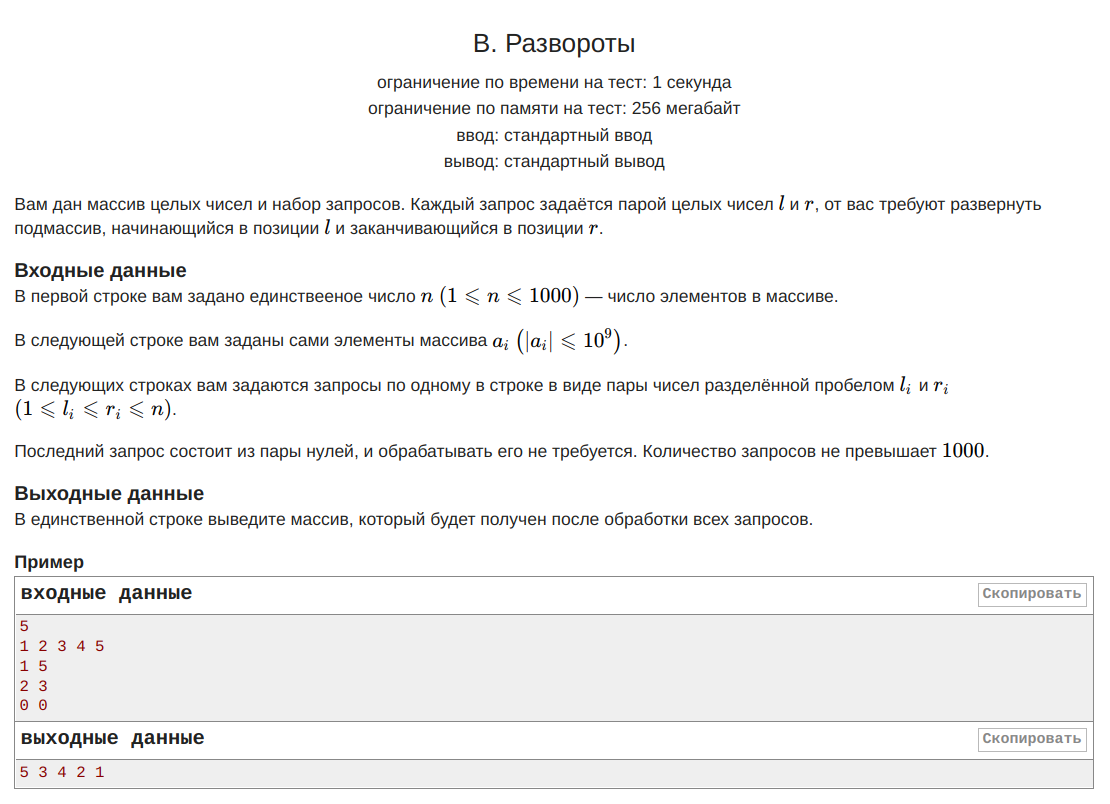
\includegraphics[width=\textwidth]{statements/Contest1B.png}
\end{center}

% Задача B
\subsubsection*{Идея решения}

В первую очередь мы вводим количество элементов в массиве, затем – последовательность в массив, а затем записываем порядки элементов, которые мы поменяем местами.
Далее мы производим операцию swap нужных элементов (не забывая увеличивать индекс начала подполследовательности и уменьшать индекс ее конца). Далее выводим отсортированную последовательность.
Сложность алгоритма $O(m \cdot n)$, где $m$ - количество запросов, а $n$ - длина разворачиваемой подпоследовательности

% {\bfseries \large Например}
% Переборное решение работает $O(n!)$, это очень долго. Использую метод динамического программирования, $dp_i$ --- это минимальное количество белочек при условии чего-то там для $i$ веточек. Это позволяет решить задачу за $O(n ^ 2)$. Дерево отрезков с отложенными обновлениями позволяет улучшить асимптотику до $O(n \cdot \log{n})$, так как все операции с деревом соврешаются за $O(\log{n})$.

\subsubsection*{Исходный код}
\lstinputlisting{src/Contest1B.cpp}

\subsubsection*{Выводы}
Задача решена.
\newline

\begin{center}
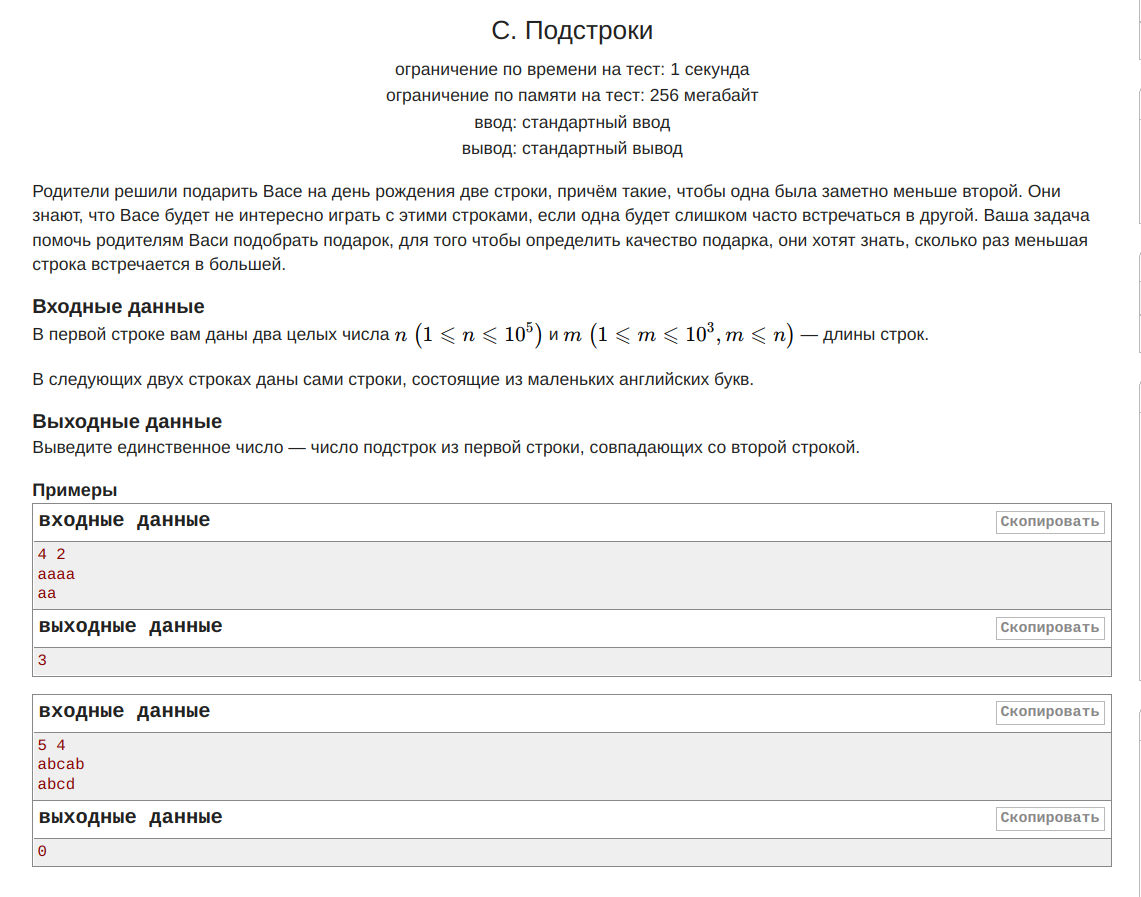
\includegraphics[width=\textwidth]{statements/Contest1C.png}
\end{center}

% Задача C
\subsubsection*{Идея решения}

Для хранения строки и подстроки будеем использовать вектор типа \textit{char}
Далее используем алгоритм прямого поиска подстроки в строке.

\newline

\textbf{Алгоритм прямого поиска подстроки в строке:} 
\begin{enumerate}
    \item i = 1
    \item сравнить i-й символ массива T с первым символом массива W
    \item совпадение → сравнить вторые символы и так далее
    \item несовпадение → i:=i+1 и переход на пункт 2
\end{enumerate}

Сложность алгоритма $O(n \cdot m)$, где $m$ - длина строки, а $n$ - длина подстроки

\subsubsection*{Исходный код}

\lstinputlisting{src/Contest1C.cpp}

\subsubsection*{Выводы}
Задача решена.

\subsubsection*{Фрагмент турнирной таблицы контеста}
\begin{center}
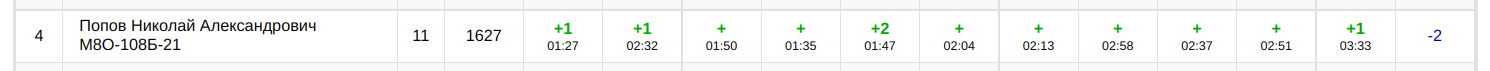
\includegraphics[width=\textwidth]{standings/Contest1Result.png}\newline\noindent
\end{center}


% CONTEST2
% БИБЛИОТЕКА С++
\subsection*{Библиотека С++}
\begin{center}
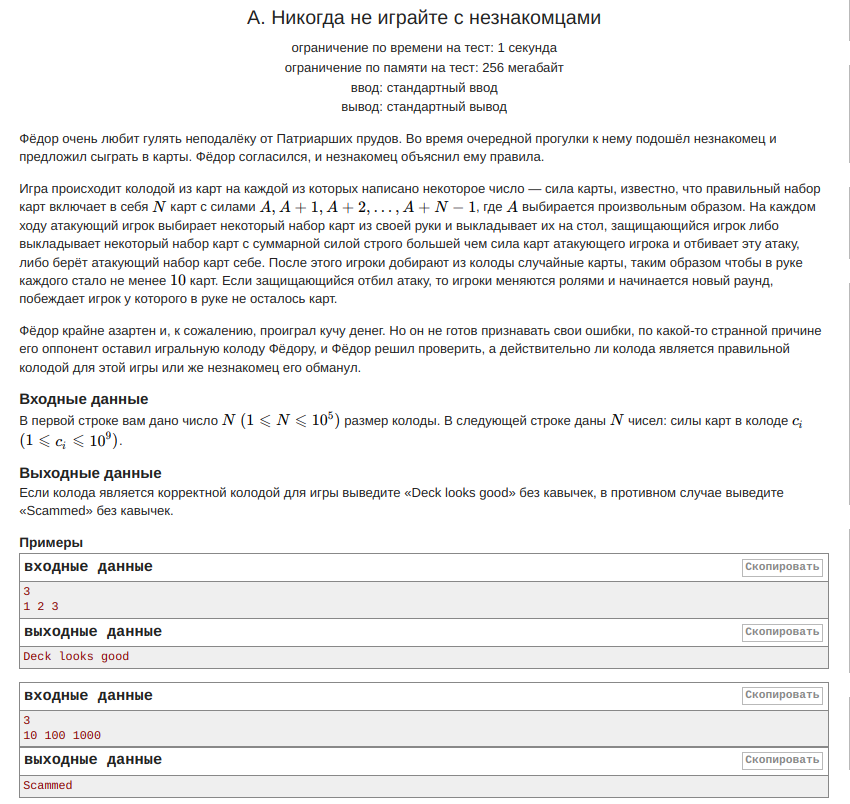
\includegraphics[width=\textwidth]{statements/Contest2A.png}
\end{center}

% Задача A
\subsubsection*{Идея решения}

В первую очередь вводим последовательность в вектор. Затем мы проверяем, заряжена ли колода в киосках: если в колоде одна карта или набор карт с значениями силы как в условии задачи (разница между соседними картами равна единице), то с колодой всё в порядке. В противном случае Федю обманули.

\subsubsection*{Исходный код}
\lstinputlisting{src/Contest2A.cpp}

\subsubsection*{Выводы}
Задача решена.
\newline

\subsubsection*{Фрагмент турнирной таблицы контеста}
\begin{center}
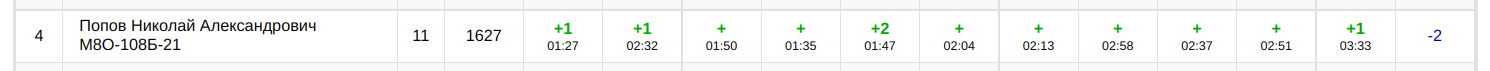
\includegraphics[width=\textwidth]{standings/Contest1Result.png}\newline\noindent
\end{center}


% CONTEST3
% Динамическое программирование
\subsection*{Динамическое программирование}
% Задача A

\begin{center}
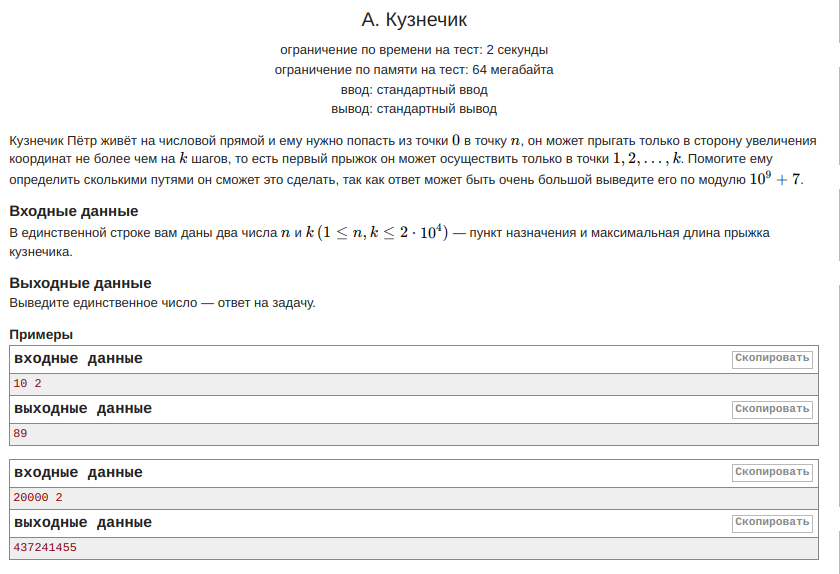
\includegraphics[width=\textwidth]{statements/Contest3A.png}
\end{center}

\subsubsection*{Идея решения}

Чтобы решить эту задачу, нам нужно составить таблицу результатов при движении на определённые координаты до значения k. Значение ячейки в 0 равно единице,
Для дальнейших ячеек необходимо добавить следующий шаг в цикле (i - j), а затем взять остаток от деления на m. После цикла выводим результат из последней ячейке массива.

\subsubsection*{Исходный код}
\lstinputlisting{src/Contest3A.cpp}

\subsubsection*{Выводы}
Задача решена.
\newline

% Задача G
\begin{center}
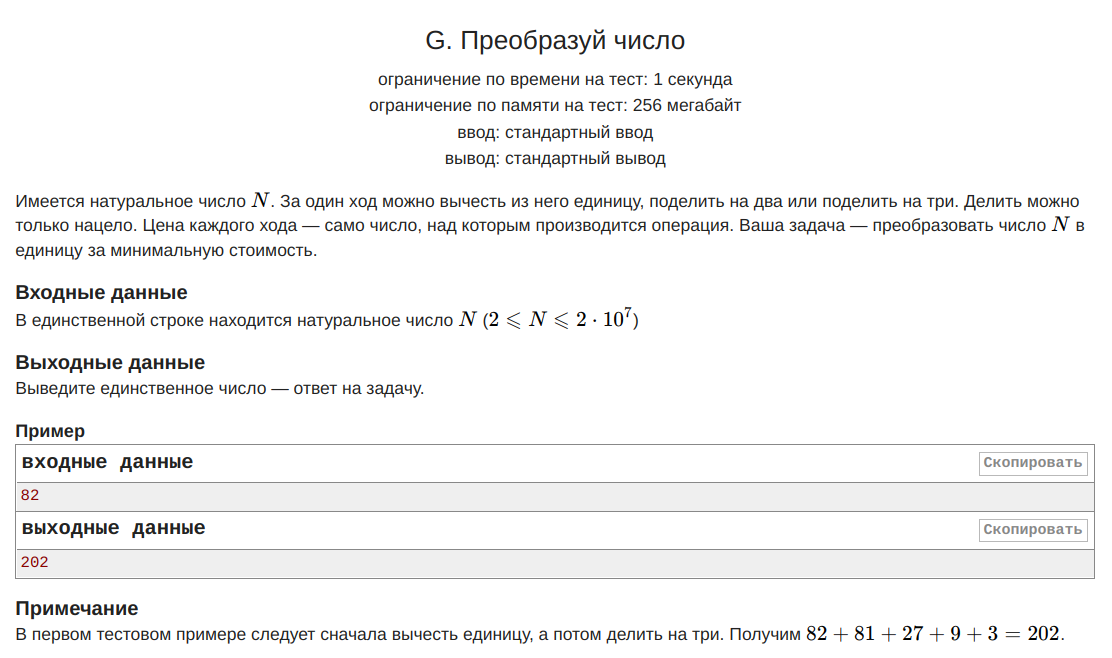
\includegraphics[width=\textwidth]{statements/Contest3G.png}
\end{center}

\subsubsection*{Идея решения}

Чтобы решить эту задачу составим таблицу из n чисел. В $i$-ой ячейке массива будем хранить количество способов получить из числа единицу.
Заполняем массив с конца, динамически добавляя к $i$-ой ячейке значения массива с индексами $i\cdot2$, $i\cdot3$, $i\cdot1$. 
После заполнения массива выводим результат - dp[1].
Сложность алгоритма - $O(n)$.

\subsubsection*{Исходный код}
\lstinputlisting{src/Contest3G.cpp}

\subsubsection*{Выводы}

Неправильный ответ на тесте 35. Ошибка из-за переполнения типа \textit{int}. Изменил тип на \textit{long long}. Задача решена.
\newline

\subsubsection*{Фрагмент турнирной таблицы контеста}
\begin{center}
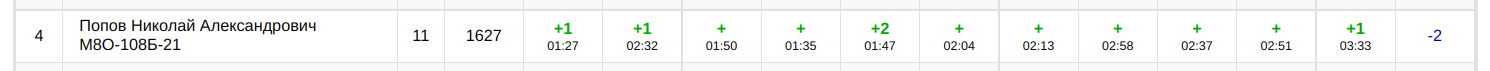
\includegraphics[width=\textwidth]{standings/Contest1Result.png}\newline\noindent
\end{center}


% CONTEST4
% Префиксные суммы, сортировка событий, два указателя
\subsection*{Префиксные суммы, сортировка событий, два указателя}
% Задача A

\begin{center}
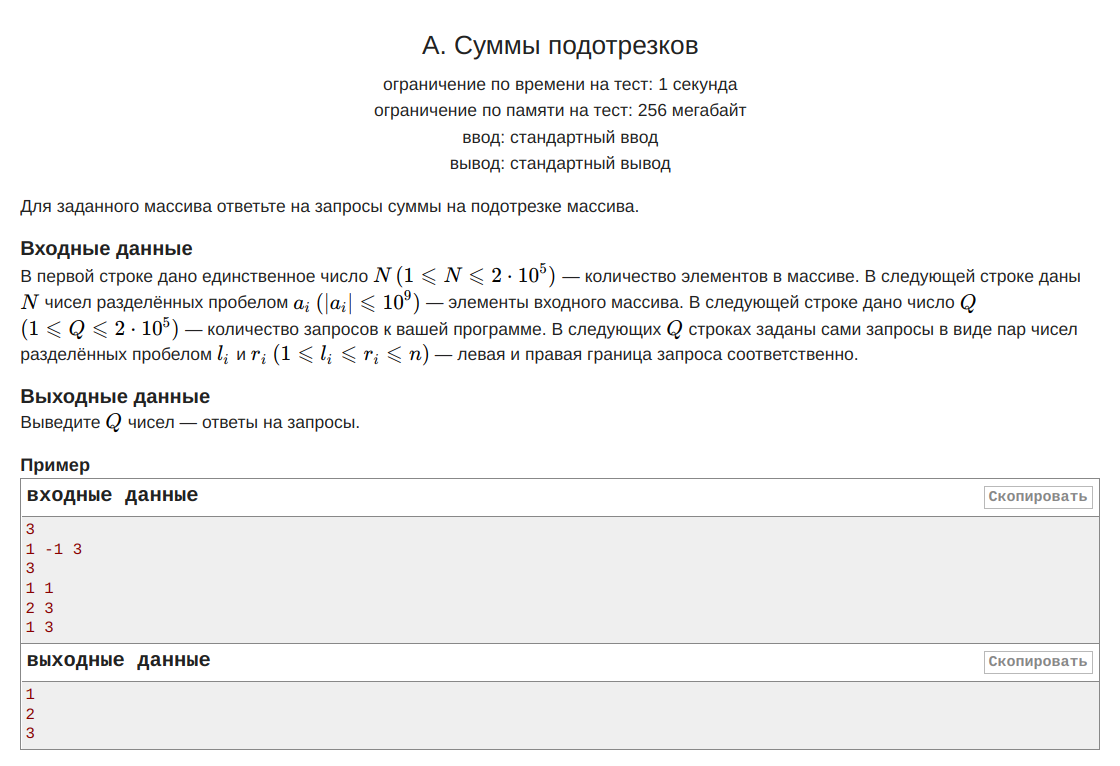
\includegraphics[width=\textwidth]{statements/Contest4A.png}
\end{center}

\subsubsection*{Идея решения}

Вводим число $n$. Затем создаем массив $a$ длины $n$ и заполняем
его.
Далее составляем массив префиксных сумм $pref$ в котором будем хранить перфиксные суммы для введенного массива.

$$pref[0] = 0,$$
$$pref[j] = pref[j - 1] + a[j]$$

Затем вводим $q$ пар чисел - левая и правая границы запроса.
Для ответа на запрос пользуемся формулой:

\begin{center}
Сумма подотрезка $[l, r] = pref[r] - pref[l - 1]$
\end{center}

Сложность заполнения масива $pref$: $O(n)$ \newline
Общая сложность алгоритма: $O(n + q)$

\subsubsection*{Исходный код}
\lstinputlisting{src/Contest4A.cpp}

\subsubsection*{Выводы}
Задача решена.
\newline

\subsubsection*{Фрагмент турнирной таблицы контеста}
\begin{center}
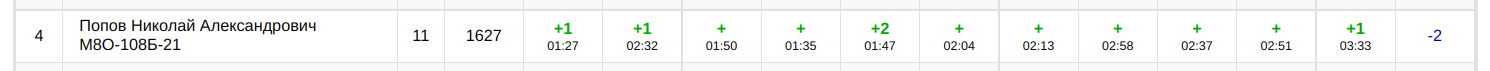
\includegraphics[width=\textwidth]{standings/Contest1Result.png}\newline\noindent
\end{center}


% CONTEST6
% Длинная арифметика
\subsection*{Длинная арифметика}
% Задача A

\begin{center}
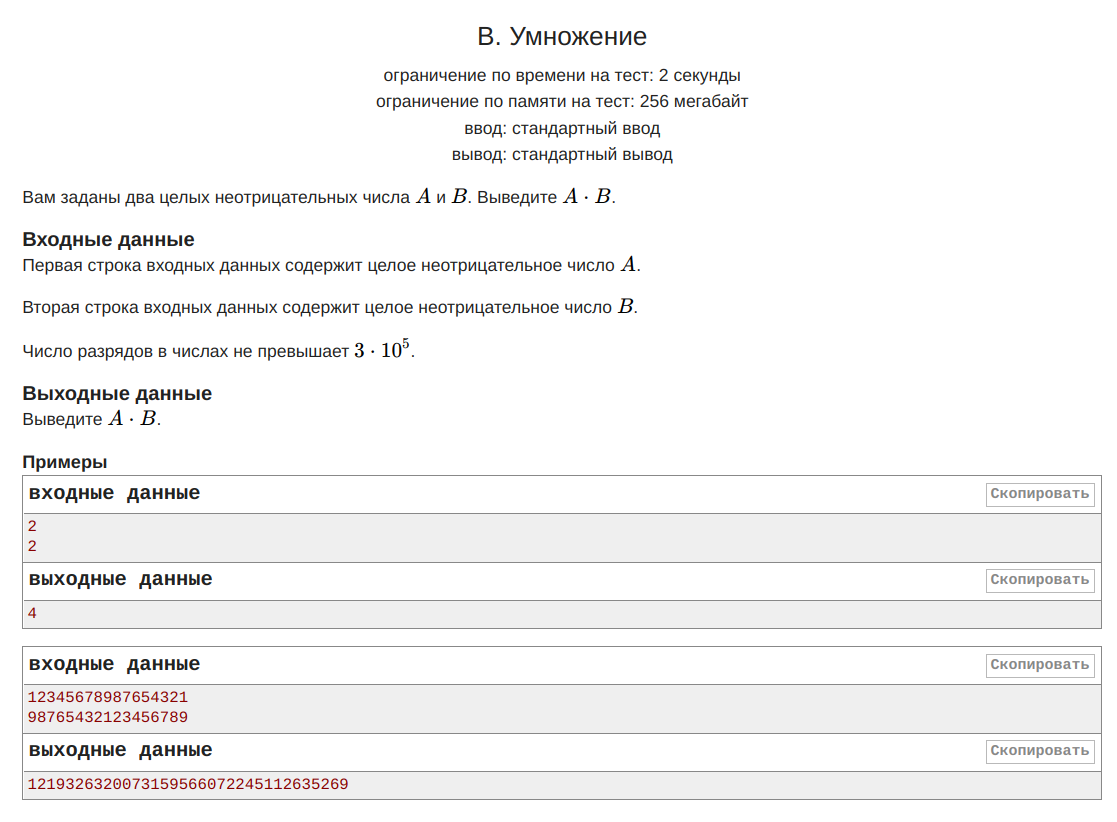
\includegraphics[width=\textwidth]{statements/Contest6B.png}
\end{center}

\subsubsection*{Идея решения}

Храним числа, которые невозможно вместить в стандартный 
целочисленный тип в виде строк. Для умножения используем быстрое 
преобразование Фурье. \newline

Сложность алогоритма: $O(n \cdot log_2 n)$ 

\subsubsection*{Исходный код}
\lstinputlisting{src/Contest6B.cpp}

\subsubsection*{Выводы}
Задача решена.

\subsubsection*{Фрагмент турнирной таблицы контеста}
\begin{center}
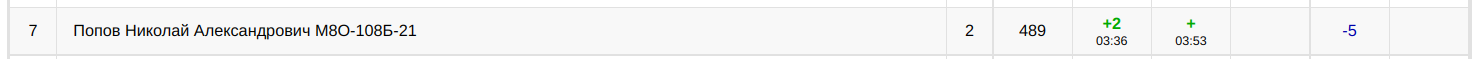
\includegraphics[width=\textwidth]{standings/Contest6.png}\newline\noindent
\end{center}


% CONTEST7
% Основы теории графов
\subsection*{Основы теории графов}

\begin{center}
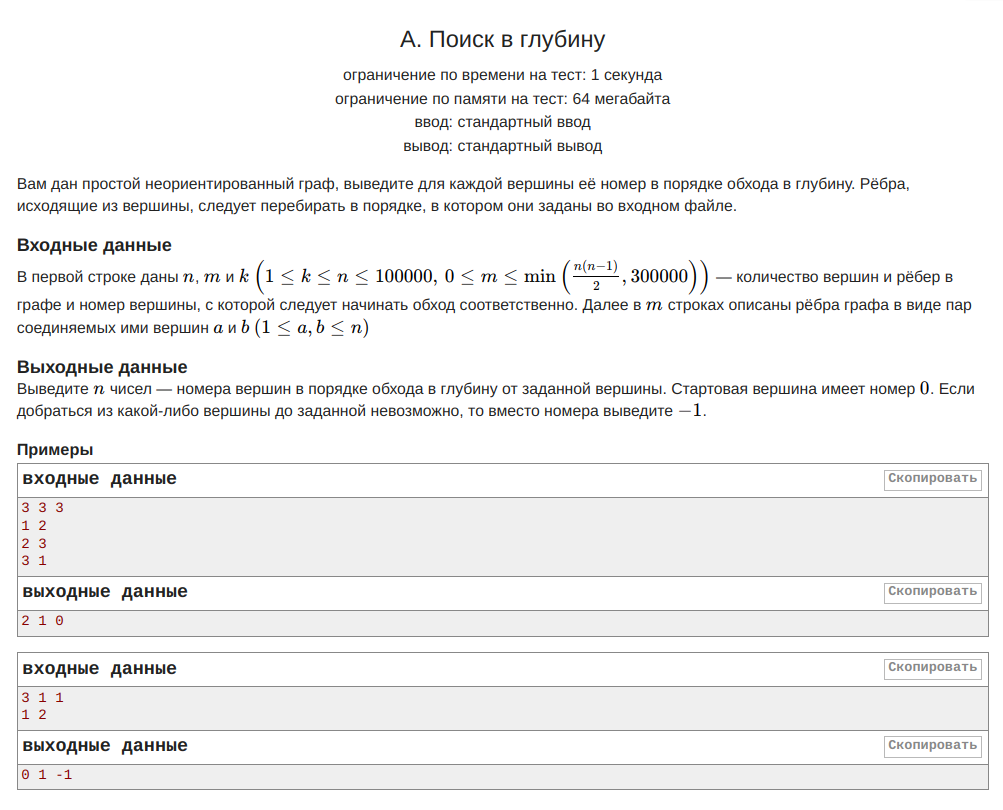
\includegraphics[width=\textwidth]{statements/Contest7A.png}
\end{center}

\subsubsection*{Идея решения}

Храним граф в виде вектора векторов целых чисел. Заполняем граф на основе входных данных. Создаем дополнительный вектор $depth$ размера $n$, в котором будем хранить глубину каждой вершины. 
При обходе в глубину прежде чем переходить к следующей вершине
инкрементируем текущую глубину и присваиваем ее соответсвующей вершине.

Сложность алгоритма: $O(n + m)$, где $n$ - число вершин, а $m$ - число ребер графа. 

\subsubsection*{Исходный код}
\lstinputlisting{src/Contest7A.cpp}

\subsubsection*{Выводы}
Задача решена.
\newline

\subsubsection*{Фрагмент турнирной таблицы контеста}
\begin{center}
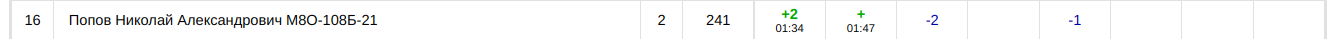
\includegraphics[width=\textwidth]{standings/Contest7.png}\newline\noindent
\end{center}


% CONTEST8
% Кратчайшие пути во взвешенных графах
\subsection*{Кратчайшие пути во взвешенных графах}

\begin{center}
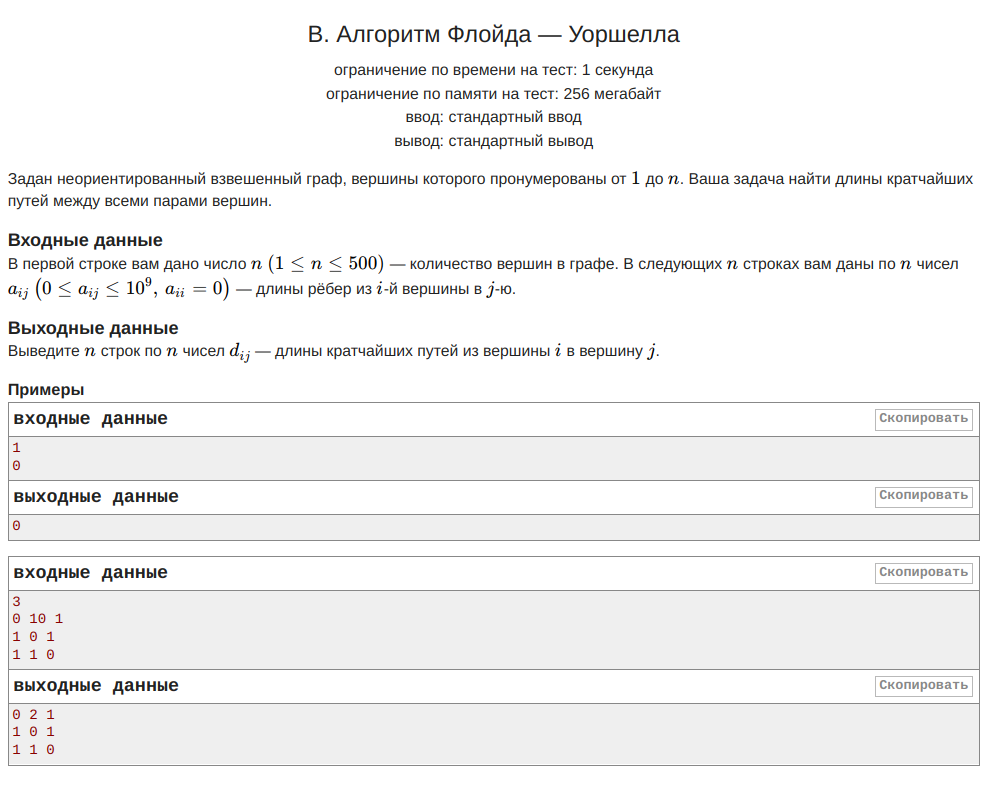
\includegraphics[width=\textwidth]{statements/Contets8B.png}
\end{center}

\subsubsection*{Идея решения}

Создадим специальную структуру для хранения ребер графа. В ней 
опишем пару вершин, которую это ребро соединяет, а также вес
этого ребра.

Храним граф в виде вектора векторов ребер. Заполняем граф на основе входных данных. Создаем таблицу для хранения кратчайших 
расстояний между вершинами. Заполняем ее, используя алгоритм
Флойда-Уоршелла. Затем выводим $n$ строк по n чисел $d_i_j$ — длины кратчайших путей из вершины $i$ в вершину $j$.

\newline
Временная сложность: $O(n^3)$ \newline
Пространственная сложность: $O(n^2)$
\newline

\subsubsection*{Исходный код}
\lstinputlisting{src/Contest8B.cpp}

\subsubsection*{Выводы}
Задача решена.
\newline

\subsubsection*{Фрагмент турнирной таблицы контеста}
\begin{center}
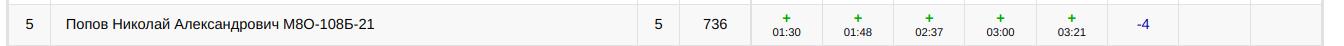
\includegraphics[width=\textwidth]{standings/Contest8.png}\newline\noindent
\end{center}



% CONTEST9
% Алгоритмы на строках
\subsection*{Алгоритмы на строках}
% Задача A

\begin{center}
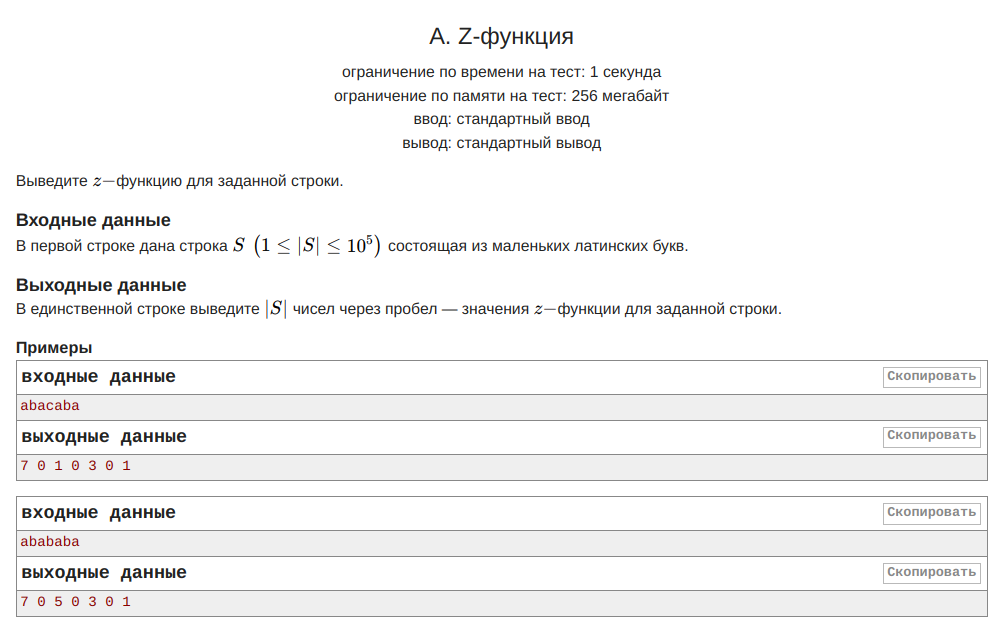
\includegraphics[width=\textwidth]{statements/Contest9A.png}
\end{center}

\subsubsection*{Идея решения}

В процессе вычисления Z-функции поддерживать последнее ненулевое найденное значение в виде границ отрезка [l;r], равного соответствующему префиксу. Под “последним” значением понимается отрезок с наибольшим r.

Таким образом, в качестве начального значения $z[i]$ можно использовать:

$$z[i] = min(z[i - l], r - i + 1)$$

После чего запускаем наивный алгоритм, пытаясь увеличить $z[i]$. Это возможно, если правая граница текущего отрезка совпадения превышает $r$, или если $i$ не входит в $[l; r]$, и вычислять $z[i]$ необходимо с нуля.

Если в результате правая граница текущего отрезка 
$(i + z[i]-1)$ превысила $r$, обновляем значения $l$ и $r$.

Сложность такого алгоритма равна $O(n)$.

\subsubsection*{Исходный код}
\lstinputlisting{src/Contest9A.cpp}

\subsubsection*{Выводы}
Задача решена.
\newline

\subsubsection*{Фрагмент турнирной таблицы контеста}
\begin{center}
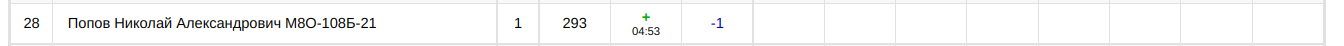
\includegraphics[width=\textwidth]{standings/Contest9.png}\newline\noindent
\end{center}





\vspace{16pt}
\pagebreak
